\section{Survey of languages with syncrhonic metathesis}\label{sec:SurLanMet}
In this section I provide a survey of
languages with synchronic metathesis.
My discussion in this section is focussed on metathesis in languages
of the greater Timor region and/or Austronesian languages.
A survey of morphological metathesis in languages beyond this scope
is given in Appendix \ref{app:MorMet}.

\begin{figure}[h]
	\caption{Synchronic metathesis in greater Timor}\label{fig:CVMetTimReg}
	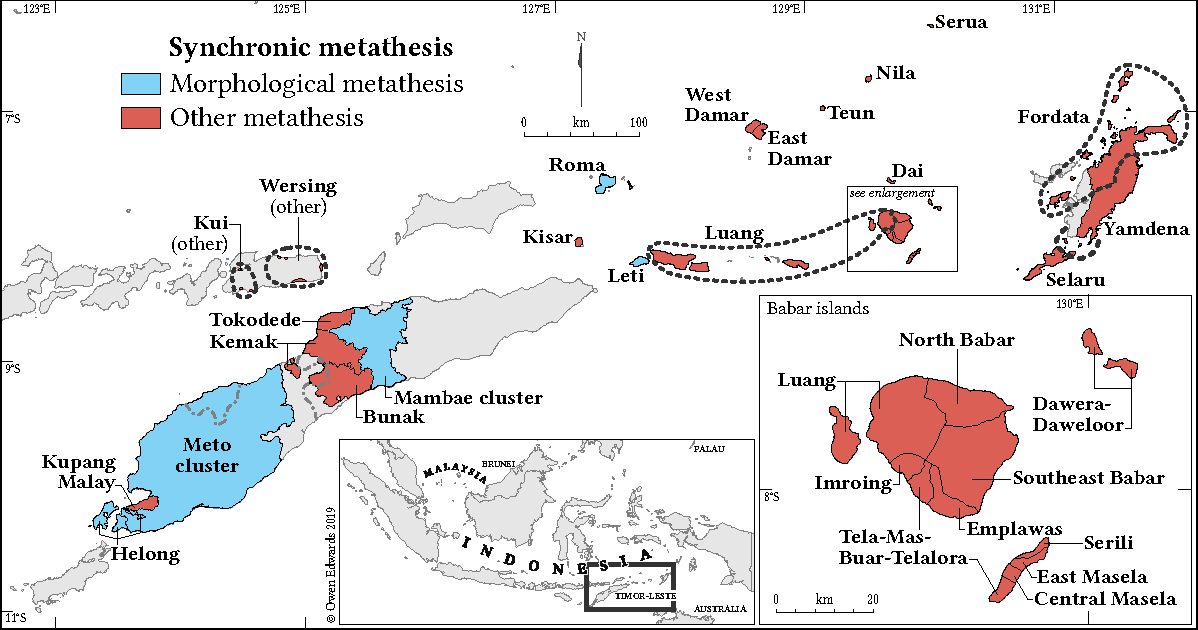
\includegraphics[width=\columnwidth]{SynchronicMetathesis.pdf}
\end{figure}

A map of languages in the greater Timor region
with synchronic metathesis is given in \frf{fig:CVMetTimReg},
based on \citet[135ff]{sc15} and my own fieldwork.
This map further marks languages in which metathesis
is known to be morphological in at least some environments.
`Other metathesis' in \frf{fig:CVMetTimReg} is used for languages
with phonologically or morphemically conditioned metathesis,
as well as for languages for which too little data is available
to determine the nature of their metathesis.

There are at least five languages of the greater Timor region
in which metathesis has a morphological function in at least some environments:
Leti (\srf{sec:Let}), Roma (\srf{sec:Rom}), Mambae (\srf{sec:Mam}),
Helong (\srf{sec:Hel}) and the Meto cluster (of which Amarasi is a member).
A further twenty or so languages have synchronic
metathesis which is phonologically conditioned,
morphemically conditioned or not yet unambiguously established as morphological.

%It is not uncommon for a single process of metathesis in a single
%language to have differently categorised in different situations.
%Thus, for instance, metathesis in Rotuman is phonologically conditioned
%in some environments, morphemically conditioned before certain affixes
%and also the sole morphological expression of indefiniteness
%(see \srf{sec:Rot} for more details).
%Similarly, metathesis in Amarasi is phonologically conditioned
%before certain enclitics and a morphological process elsewhere. 

I begin my discussion in this section with Kwara'ae (\srf{sec:Kwa})
and Rotuman (\srf{sec:Rot}), both of which are spoken in the Pacific
and outside the greater Timor region.
I then discuss cases of synchronic metathesis
in the greater Timor region starting with the non-Austronesian
languages Wersing (\srf{sec:Wer}) and Bunak (\srf{sec:Bun}).
After this I discuss synchronic metathesis among Austronesian
languages of the greater Timor region moving geographically
closer to Meto with each language discussed.

Before proceeding with the discussion
it is necessary to clarify two points.
Firstly, in some cases I give isolated examples of metathesis
of the type X {\ra} Y
(e.g. Rotuman \it{ho\tbr{sa}} {\ra} \it{ho\tbr{as}}
`flower' on page \pageref{ex:VCV->VVC})
or X + Z {\ra} YZ (e.g. Luang \it{ʔer\tbr{nu}} + \it{la}
{\ra} \it{ʔer\tbr{un}la} `go down to' on page \pageref{ex:LuaMet}).
In all such cases the form before the arrow is
a form which surfaces in certain contexts.
Thus, all putative examples of metathesis throughout this section
are based on true surface alternations.\footnote{
		Readers who find a particular analysis involving metathesis
		unconvincing should consult the original sources for full
		discussion and justification.}

Secondly, in such examples the form
before the arrow is the presumed underlying form.
The identification of underlying forms follows that of the sources,
which in turn is usually based on phonological and morphological analysis.
However, I do not usually repeat here the evidence for this analysis.
Interested readers should consult the original sources.
Again, in all cases the presumed underlying form
is a form which surfaces in certain contexts, as discussed above.